% -------------------------------------------------------------------------------- %

\begin{exercise}[Exercise 3.17]

What is the Bellman equation for action values, that is, for $q_\pi$? It must give
the action value $q_\pi(s,a)$ in terms of the action values, $q_\pi(s',a')$, of
possible successors to the state-action pair $(s,a)$. \\
\textit{Hint:} The backup diagram below corresponds to this equation.
Show the sequence of equations analogous to (3.14), but for action values.

\begin{figure}[H]
    \centering
    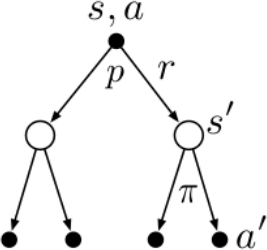
\includegraphics[width = 0.5 \textwidth]{3.17.png}
\end{figure}

\end{exercise}

% -------------------------------------------------------------------------------- %

\begin{solution}

\begin{align*}
  q_\pi(s,a) \ &\dot = \ \E_\pi[G_t | S_t = s, A_t = a] \\
  &= \E_\pi[R_{t+1} +  \gamma G_{t+1} | S_t = s, A_t = a] \\
  &= \sum_{s',r} p(s',r|s,a)\left[r + \gamma \E_\pi[G_{t+1} | S_{t+1} = s']\right] \\
  &= \sum_{s',r} p(s',r|s,a)\left[r + \gamma \sum_{a'} \pi(a'|s')\E_\pi[G_{t+1} | S_{t+1} = s', A_{t+1} = a']\right] \\
  &= \sum_{s',r} p(s',r|s,a)\left[r + \gamma \sum_{a'} \pi(a'|s') q_\pi(s',a')\right] \\
\end{align*}

\end{solution}

% -------------------------------------------------------------------------------- %
